\documentclass[aspectratio=169]{beamer}

\usetheme{Boadilla}
\usefonttheme{professionalfonts}
\usefonttheme{structuresmallcapsserif}

\usepackage{amsmath, latexsym, amsfonts, amssymb, amsthm}
\newtheorem{remark}[theorem]{Remark}
\newtheorem{observation}[theorem]{Observation}

\usepackage[T1]{fontenc}
\usepackage{garamondx}
\usepackage[garamondx,cmbraces]{newtxmath}
\usepackage{listings}

\setbeamertemplate{section page}
{
    \begin{centering}
    \usebeamerfont{section title}\usebeamercolor[fg]{section name}\sectionname~\MakeUppercase{\romannumeral\insertsectionnumber}\\
    \begin{beamercolorbox}[sep=12pt,center]{part title}
    \usebeamerfont{section title}\insertsection\par
    \end{beamercolorbox}
    \end{centering}
}
\defbeamertemplate{section in toc}{sections numbered roman}{%
  \leavevmode%
  \MakeUppercase{\romannumeral\inserttocsectionnumber}.\ %
  \inserttocsection\par}
\setbeamertemplate{section in toc}[sections numbered roman]

\title[DKRV14 and DMS14]{Unit volume Liouville measure on the sphere with $(\gamma,\gamma,\gamma)$-insertions: the link between two constructions}
\author[Yichao Huang]{Yichao Huang$^{[ENS]}$, joint with Juhan Aru$^{[ETH]}$, Xin Sun$^{[MIT]}$}
\date[IH\'ES, 17 May 2016]{}

\begin{document}
\AtBeginSection{\frame{\sectionpage}}

\begin{frame}
\titlepage
\end{frame}

\begin{frame}
\frametitle{Introduction}
\framesubtitle{Motivation: Liouville Quantum Gravity}
Two constructions of random measures on the sphere by David$^\circ$, Duplantier$^\bullet$, Kupiainen$^\circ$, Miller$^\bullet$, Rhodes$^\circ$, Sheffield$^\bullet$, Vargas$^\circ$.\\
$\circ=[DKRV14]$: explicit formul\ae~for correlation functions, $n\geq 3$ insertions of arbitrary weights, suitable for compact surfaces of all genus.\\
$\bullet=[DMS14]$: $n\leq 2$ insertions with same weight, metric in the $\gamma=\sqrt{8/3}$ case, SLE/GFF coupling, suitable for non-compact surfaces.\\
~\\
Goal of $[AHS15]$: find a link between these two constructions.

\end{frame}

\begin{frame}
\frametitle{Outline}
\tableofcontents
\end{frame}


\section{Conformal embedding}

\begin{frame}
\frametitle{M\"obius transformations}
\framesubtitle{as the automorphism group of the Riemann sphere}
\begin{definition}
A (conformal) automorphism $\varphi$ of the complex plane $\mathbb{C}$ writes
$$\varphi: z\mapsto\frac{az+b}{cz+d}$$
with $a,b,c,d\in\mathbb{C}$, $ad-bc=1$.
\end{definition}
Exercice 1: give all $\varphi$ such that $\varphi(0)=0, \varphi(1)=1, \varphi(\infty)=\infty$.\\
Exercice 2: give all $\varphi$ such that $\varphi(0)=0, \varphi(\infty)=\infty$.
\end{frame}

\begin{frame}
\frametitle{Embedding with \underline{three} marked points}
\framesubtitle{as a well-defined random measure}
\begin{columns}[T]
\begin{column}{.54\textwidth}
~\\
~\\
Take a large random planar map with chosen marked points $(z_1,z_2,z_3)$ and some conformal structure.\\
We ``embed'' this map on the sphere by sending conformally $(z_1,z_2,z_3)$ to $(0,1,\infty)$.\\
There is a unique way to do it -- the limiting measure should be described by a random measure.\\
~\\
Conjecture: choose the three marked points uniformly among all vertices, convergence to Liouville measure with three insertions of weight $\gamma$.
\end{column}
\begin{column}{.44\textwidth}
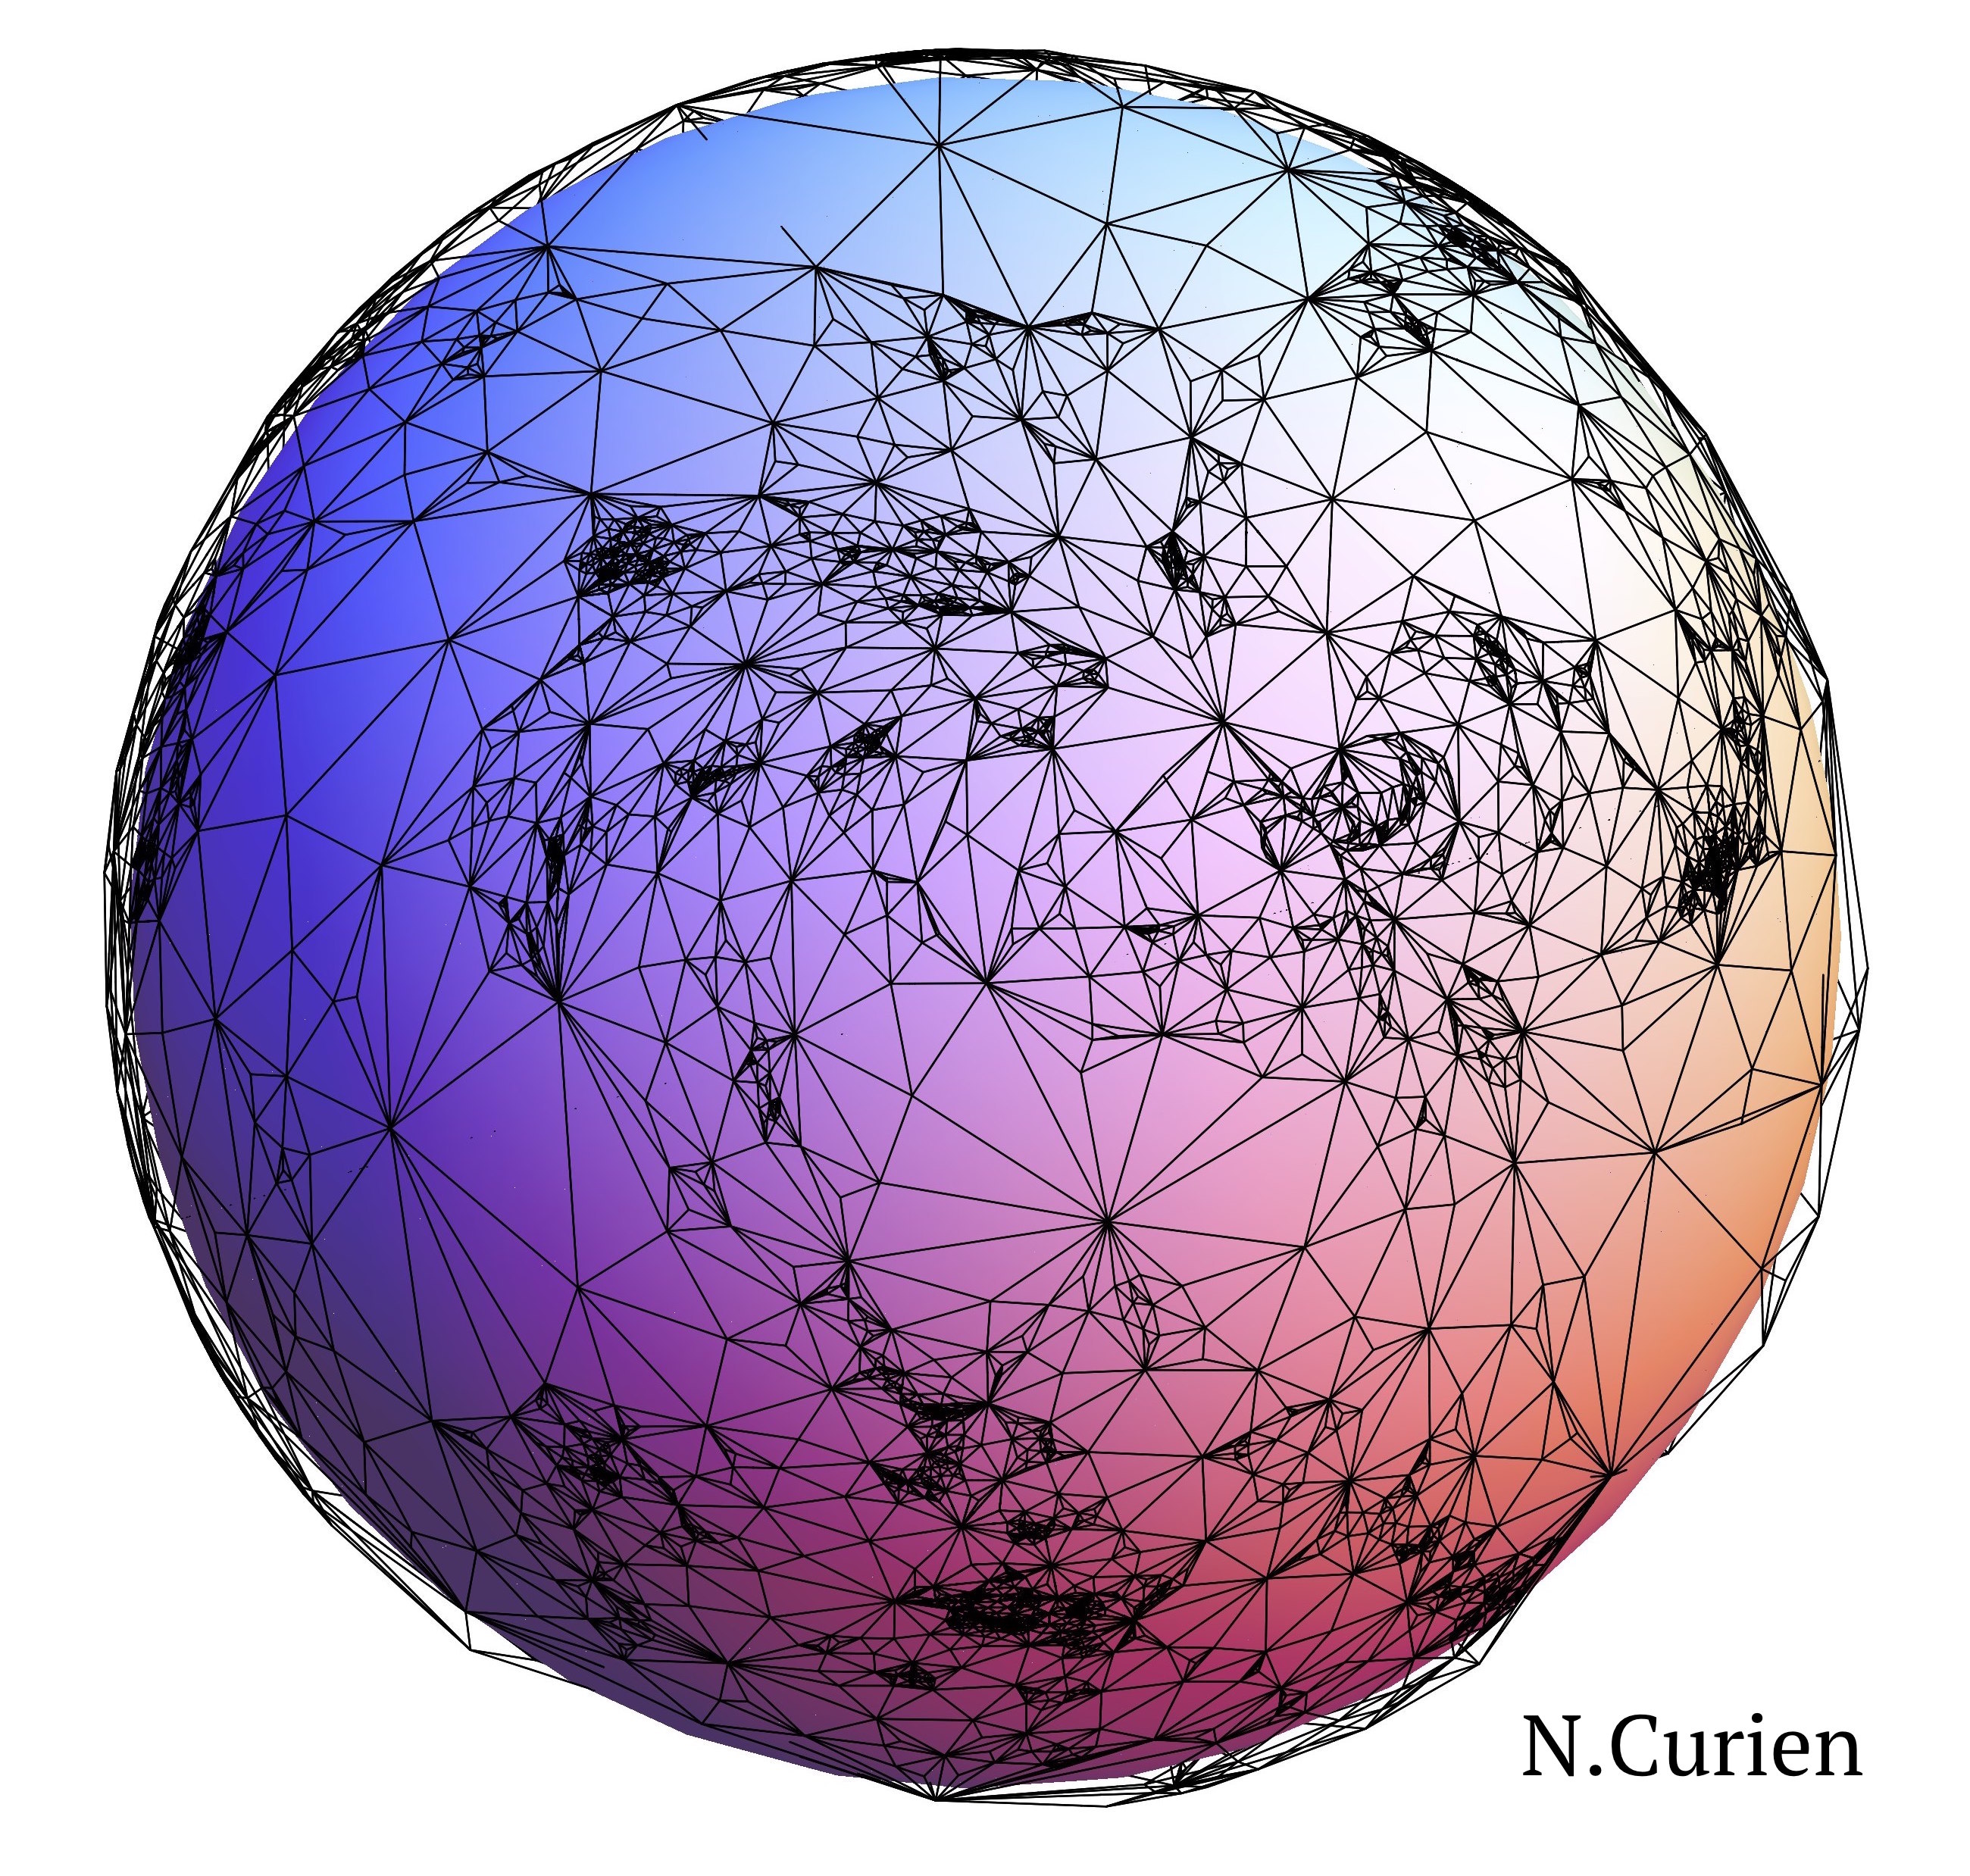
\includegraphics[width=\textwidth]{nc.jpg}
\end{column}
\end{columns}
\end{frame}

\begin{frame}
\frametitle{Embedding with \underline{two} marked points}
\framesubtitle{as an equivalence class of random measures}
Imagine instead we only consider two points $(z_1,z_2)$ and we map them to $(0,\infty)$.\\
The mapping is ill-defined! We make use of the following equivalence class:
\begin{definition}[A quotient space $\mathcal{Q}$]
Two (random) measures with marked points $(D,\mu,s_1,\dots,s_n)$ and $(D',\nu,t_1,\dots,t_n)$ are said equivalent if there is a (random) conformal map $\varphi$ from $D$ to $D'$ that maps $(s_1,\dots,s_n)$ to $(t_1,\dots,t_n)$ and such that $\varphi_*(\mu)=\nu$; $\varphi_*$ is the pushforward defined by $\varphi_*(\mu)(A)=\mu(\varphi^{-1}(A))$.
\end{definition}
In particular, if we fix $\mathbb{C}$ with two marked points $(0,\infty)$, we get a family of (random) measures defined \emph{modulo a dilatation}. One should describe this limit using a construction that is not sensible to the action of a certain subgroup of the M\"obius group (here, the dilatations).
\end{frame}


\section{Two constructions}

\begin{frame}
\frametitle{The DKRV definition}
\framesubtitle{of the unit volume Liouville measure with $n\geq 3$ insertions}
\begin{definition}[Unit volume Liouville measure]
Let $g$ be a metric on the sphere. Let $X_g$ be a whole plane GFF such that $\int_{\mathbb{R}^2}X_g(z)dg=0$.
Consider
$$X_L=X_g(z)+\sum_i\alpha_i\ln|z-z_i|$$
and let $Z_\gamma(\mathbb{R}^2)=\int_{\mathbb{R}^2}e^{\gamma X_L(z)}d\lambda_g$ the volume form associated with $X_L$.\\
The law of the unit volume Liouville measure is given by
$$\mu(A)=\int_{A}e^{\gamma X_U(z)}d\lambda_g$$
where $X_U=X_L-\frac{1}{\gamma}\ln Z_\gamma(\mathbb{R}^2)$ under the measure $Z_\gamma(\mathbb{R}^2)^{\frac{2Q-\sum_i\alpha_i}{\gamma}}d\mathbb{P}_{X_g}$.
\end{definition}
\end{frame}

\begin{frame}
\frametitle{The DMS equivalence class of random measures}
\framesubtitle{with two $\gamma$-insertions at $0$ and $\infty$}
\begin{definition}[Bessel process encoding]
Every distribution on $\mathbb{C}$ can be decomposed into two parts:\\
-- the radial part: average on circles $\partial B(0,r)$;\\
-- the lateral noise part: fluctuation on each circles.\\
~\\
Let $\delta=4-8/\gamma^2$ and $\nu^{BES}_\delta$ the Bessel excursion measure of dimension $\delta$.\\
We sample the radial part $R$ in the following way:\\
1. Sample a Bessel excursion $\mathfrak{e}$ w.r.t. $\nu^{BES}_\delta$;\\
2. Reparametrizing $\frac{1}{\gamma}\log\mathfrak{e}$ to have unit quadratic variation.\\
Add (independently) the lateral noise $N$ part by projection.\\
~\\
This will give us a distribution (in fact, a Gaussian field) \emph{defined modulo dilatation}. Take the exponential: we get the equivalence class of random measures with two $\gamma$-insertions at $0$ and $\infty$.
\end{definition}
\end{frame}


\section{Theorem and consequences}

\begin{frame}
\frametitle{Main theorem of [AHS15]}
\framesubtitle{From DMS14 to DKRV14}
For better comprehension, we state the theorem in plain words.
\begin{theorem}[AHS15]
Take the sphere, or the whole plane.\\
1. Consider a measure in the DMS equivalence class with two $\gamma$-insertions at $0$ and $\infty$;\\
2. Choose a third point $z$ w.r.t. this measure;\\
3. Use a conformal map that shifts $(0,z,\infty)$ to $(0,1,\infty)$;\\
4. Push-forward the chosen measure in the DMS class by this conformal map;\\
5. We get DKRV measure with three $\gamma$-insertions at $0$, $1$ and $\infty$!
\end{theorem}
Attention! It is not trivial to describe the random conformal map in step 3.
\end{frame}

\begin{frame}
\frametitle{Consequence}
\framesubtitle{From DKRV14 to DMS14\dots}
\begin{remark}[Consequence]
1. Take DKRV measure with three $\gamma$-insertions at $0$, $1$ and $\infty$;\\
2. Forget about the point $1$, and pass to the quotient space $\mathcal{Q}$;\\
3. We get the DMS equivalence class with two $\gamma$-insertions at $0$ and $\infty$.
\end{remark}
\end{frame}

\begin{frame}
\frametitle{Thanks!}
\begin{block}{Isaac Newton Institute for Mathematical Sciences}
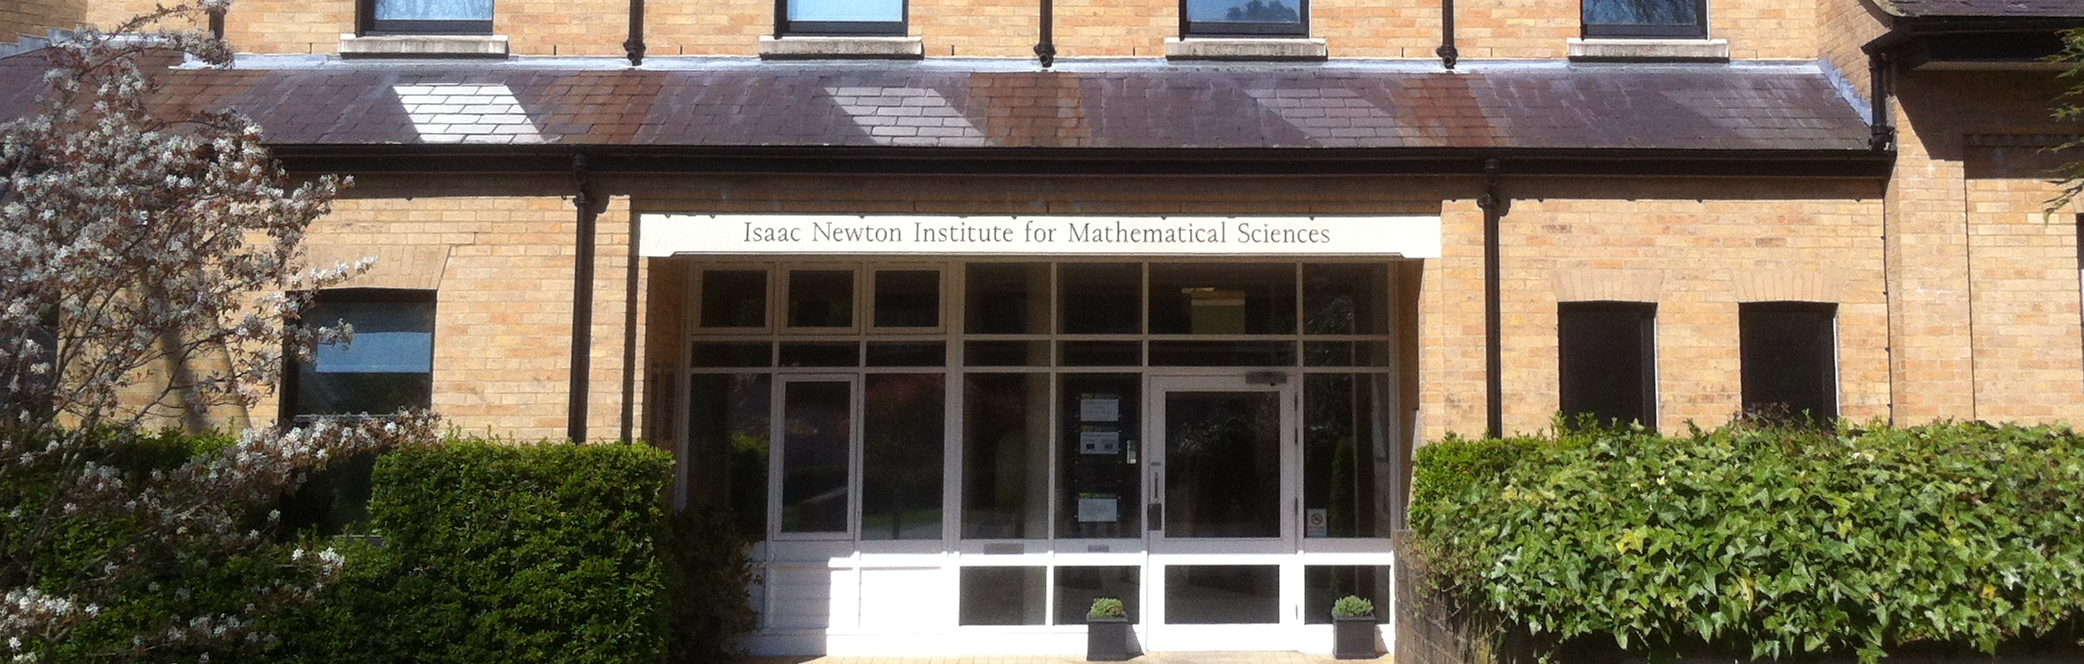
\includegraphics[width=\textwidth]{INI.png}
\end{block}
\end{frame}

\end{document}
